\documentclass[a4paper]{article}

\usepackage[pdftex]{graphicx}
\usepackage[margin=3cm]{geometry}
\usepackage{verbatim,moreverb,amssymb,amsmath}


\newcounter{question}
\newcommand{\question}[1]{\refstepcounter{question}\section*{Question~\thequestion~~~\small\emph{(#1)}}}
\renewcommand*\thequestion{\arabic{question}}


\begin{document}

\pagestyle{empty}
\thispagestyle{empty}



\noindent
\begin{minipage}{\columnwidth}
  \centering
  \Large
  DA4002 (HT13) Halmstad University\\
  Introduction to Algorithms, Data Structures, and Problem Solving\\[3\baselineskip]
  \Huge
  Written Exam\\
  \Large
  Friday, November 1, 2013\\[2\baselineskip]
  Examiner: Roland Philippsen
\end{minipage}

\vfill

\noindent
\begin{center}
\fbox{
  \begin{minipage}{0.8\columnwidth}
    \textbf{Student Name:}\\[3\baselineskip]
  \end{minipage}
}
\end{center}

\vfill



\section*{Rules}

Aside from the obvious rules of conduct exams (e.g.\ no chatting):

\begin{itemize}
\item
  \textbf{No computing devices} (laptops, phones, calculators, \emph{etc}).
\item
  \textbf{No books or printouts} except for non-electronic dictionaries.
\item
  \textbf{Allowed hand-written notes}: two sheets of A4 paper (front and back).
\end{itemize}



\section*{General Guidelines}

\begin{itemize}
\item
  \textbf{Read carefully} and pace yourself.
  You can solve the problems in any order you want, but later problems may be easier to solve after you have answered the preceding questions.
\item
  \textbf{Write clearly} and draw clear diagrams.
  If you need to correct a mistake, then cleanly cross out the wrong answer and clearly indicate where the correction can be found.
\item
  \textbf{Indicate the question number} for each of your answers.
  If a question has sub-questions, indicate the sub-question number after the main question number, separated by a dot.
  For example, question 3 has 4 sub-questions, and their answers should be numbered 3.1, 3.2, 3.3, and 3.4.
\end{itemize}



\pagebreak
\pagestyle{plain}
\thispagestyle{plain}
\setcounter{page}{1}



\question{6 points}

In the following table, match the data structure names with the diagrams \textbf{(A, B, or C)}, and the code segments \textbf{(X, Y, or Z)}.

\vfill

\begin{center}
  \begin{tabular}{|l|*2{p{0.25\columnwidth}|}}
    \hline
    \emph{data structure} & \emph{diagram (A, B, or C)} & \emph{code (X, Y, or Z)} \\
    \hline
    simply linked list & & \\
    \hline
    doubly linked list & & \\
    \hline
    simply linked circular list & & \\
    \hline
    doubly linked circular list & & \\
    \hline
    binary tree & & \\
    \hline
    sibling-child tree & & \\
    \hline
  \end{tabular}
\end{center}

\vfill

\begin{center}
  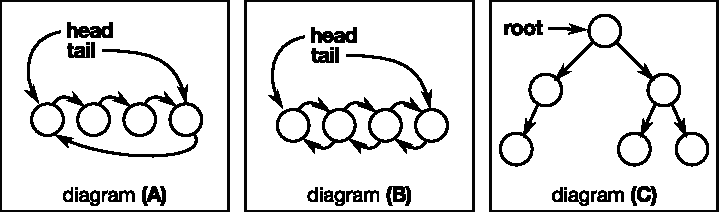
\includegraphics[width=0.8\columnwidth]{q1diag.pdf}
\end{center}

\vfill

\noindent
\begin{minipage}{0.42\columnwidth}
  \fbox{\begin{minipage}{\columnwidth}
      code segment \textbf{X}:
      \small
      \verbatiminput{q1x.c}
  \end{minipage}}
  \fbox{\begin{minipage}{\columnwidth}
      code segment \textbf{Z}:
      \small
      \verbatiminput{q1z.c}
  \end{minipage}}
\end{minipage}
\hfill
\fbox{\begin{minipage}{0.52\columnwidth}
    code segment \textbf{Y}:
    \small
    \verbatiminput{q1y.c}
\end{minipage}}

\clearpage


\question{6 points}

Give them recursive code for the coin change problem, let them develop and fill out the DP variant.



\clearpage

\question{6 points}

\begin{enumerate}
\item
  What is the the Big-Oh $O(N)$ expressions for the following runtime formula $T_1(N)$?
  \begin{equation*}
    T_1(N) = N \left( 12\log N + \sum_{i=1}^Ni \right) + 0.1 N^2
  \end{equation*}
\item
  What is the the Big-Oh $O(N)$ expressions for the following runtime formula $T_2(N)$?
  \begin{equation*}
    T_2(N) =
    \begin{cases}
      1          & \text{for} N \leq 1 \\
      2 T_2(N/2) & \text{otherwise}
    \end{cases}
  \end{equation*}
\item
  What is the Big-Oh $O(N)$ expression for the runtime $T_3(N)$ of the following code segment?\\[1.5\baselineskip]
  \fbox{\begin{minipage}{0.8\columnwidth}
      \small
      \verbatiminput{q2a.c}
  \end{minipage}}\\[2\baselineskip]
\item
  What is the Big-Oh $O(N)$ expression for the runtime $T_4(N)$ of the following code segment?\\[1.5\baselineskip]
  \fbox{\begin{minipage}{0.8\columnwidth}
      \small
      \verbatiminput{q2b.c}
  \end{minipage}}
\end{enumerate}



\clearpage

\question{6 points}

Do a bunch of runtime estimates given big-Oh expressions.

\vfill

\noindent
\begin{tabular}{|l|r|r|r|r|r|r|r|r|r|r|r|r|r|r|r|}
  \hline
  $x=$   & 0 & 1 & 2 &  3 &  4 &   5 &   6 &   7 &   8 &   9 &   10 &   11 &   12 &   13 &    14 \\
  $x^2=$ & 0 & 1 & 4 &  9 & 16 &  25 &  36 &  49 &  64 &  81 &  100 &  121 &  144 &  169 &   196 \\
  $x^3=$ & 0 & 1 & 8 & 27 & 64 & 125 & 216 & 343 & 512 & 729 & 1000 & 1331 & 1728 & 2197 &  2744 \\
  $2^x=$ & 1 & 2 & 4 &  8 & 16 &  32 &  64 & 128 & 256 & 512 & 1024 & 2048 & 4096 & 8192 & 16384 \\
  \hline
\end{tabular}



\clearpage

\question{6 points}

Give an adjacency matrix, let them draw the graph, describe Dijkstra, let them run it on the graph they drew.



\clearpage

\question{6 points}

Hmm\ldots unbalanced tree problem is always a good one, and I don't think I have trees yet.
Or something to do with tree traversal\ldots

Or some tricky questions, like someone suggests to sort a linked list in order to be able to use binary search (does not make sense because linked lists do not provide random access), someone suggests to sort an array before looking for pairs of values that sum to a divisor of a given number (I don't think sprting here makes sense because youhave to try all combinations anyway), but also include two sensible suggestions, such as using level-order traversal to save a balanced binary search tree (as opposed to in- or post-order traversal which makes it unbalanced when you load it back).

\end{document}
